\subsection{Object Transformers VM Implementation}

\begin{frame}[t]{Transforming objects in the GC}%{A Sub-title is optional}
Happens in two steps \\
\begin{itemize}
\item Garbage collector creates an additional empty copy for updated objects
\item Walk through and transform all these objects
\end{itemize}
\vspace*{2ex}
Example
\vspace*{-3ex}
\begin{center}
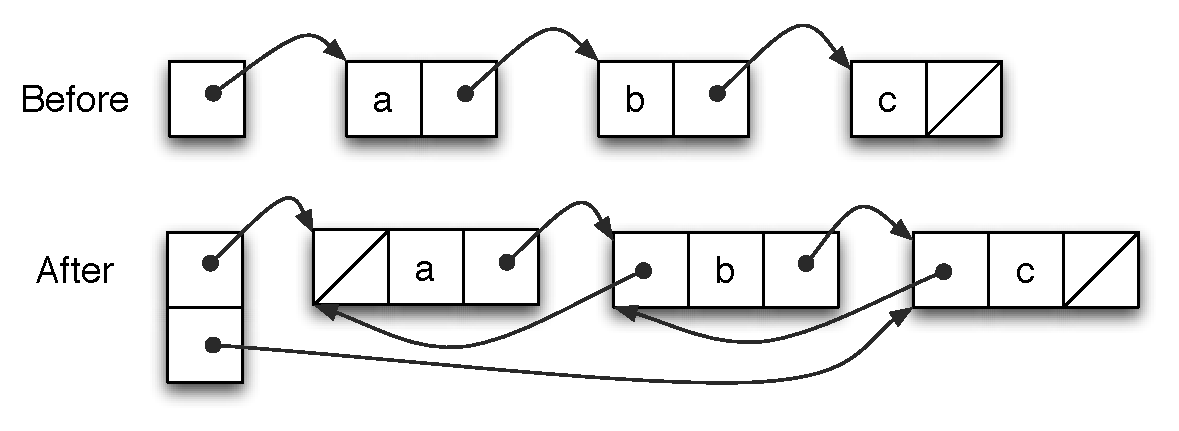
\includegraphics[scale=0.6]{images/singly-doubly/linked-lists-without-gc}%
\end{center}
\end{frame}

% \begin{frame}[fragile]{Jvolve GC}%{A Sub-title is optional}
% \begin{columns}[c]
% \begin{column}{0.67\paperwidth}
% \only<1>{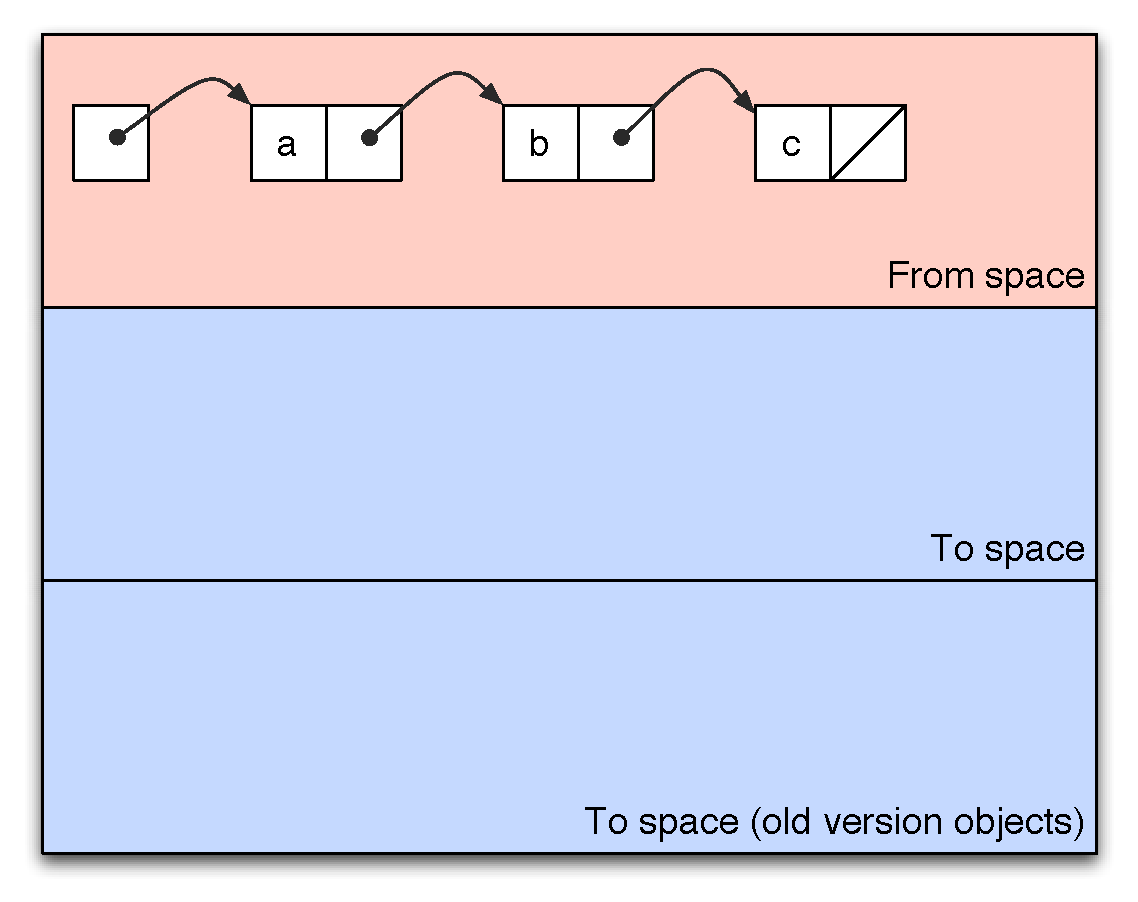
\includegraphics[scale=0.45]{images/singly-doubly/before-gc-copy}}%
% \only<2>{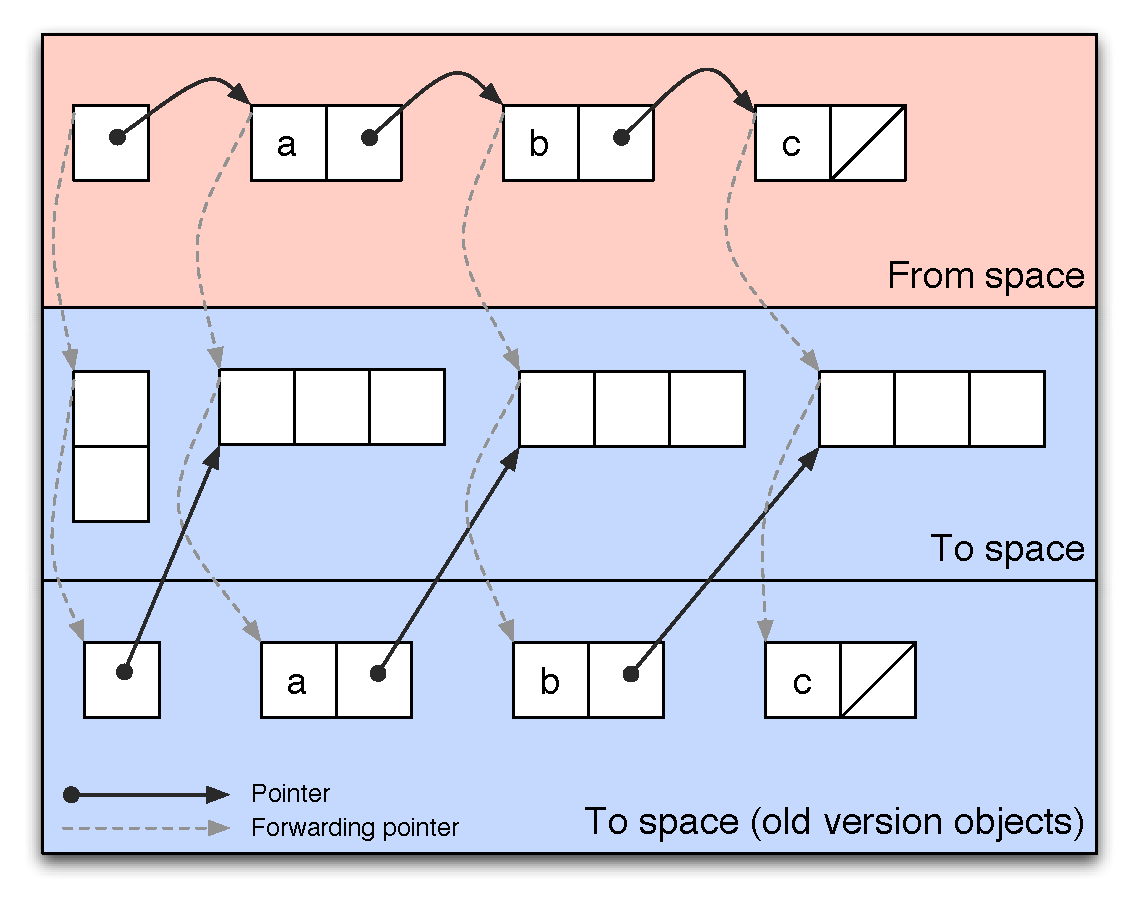
\includegraphics[scale=0.45]{images/singly-doubly/singly-doubly}}%
% \only<3>{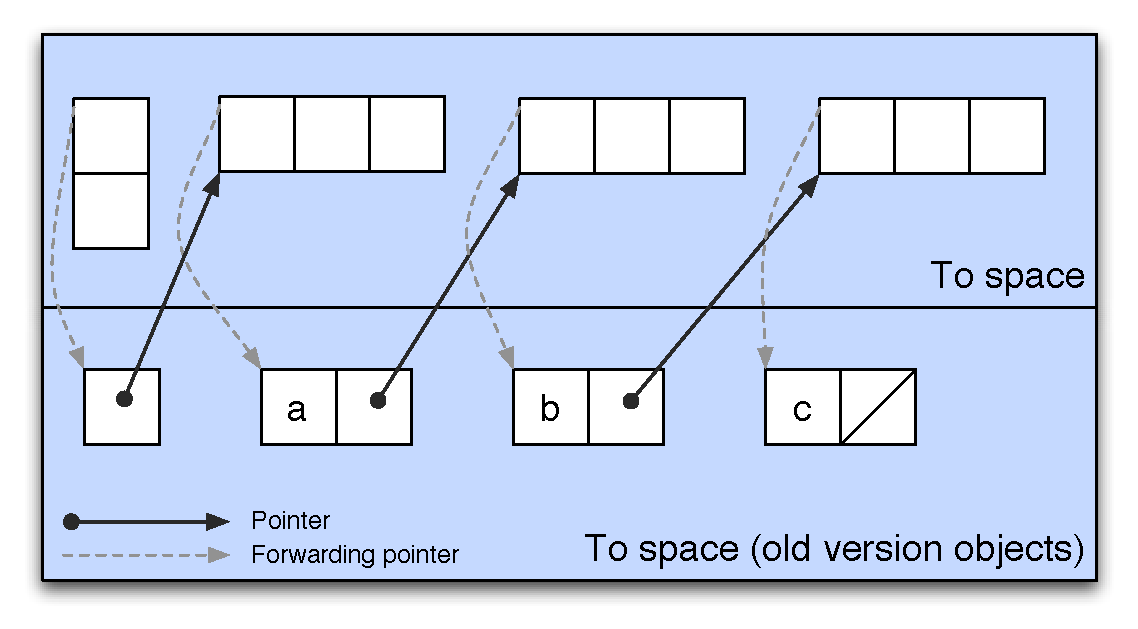
\includegraphics[scale=0.45]{images/singly-doubly/singly-doubly-before-transform}}%
% \only<4>{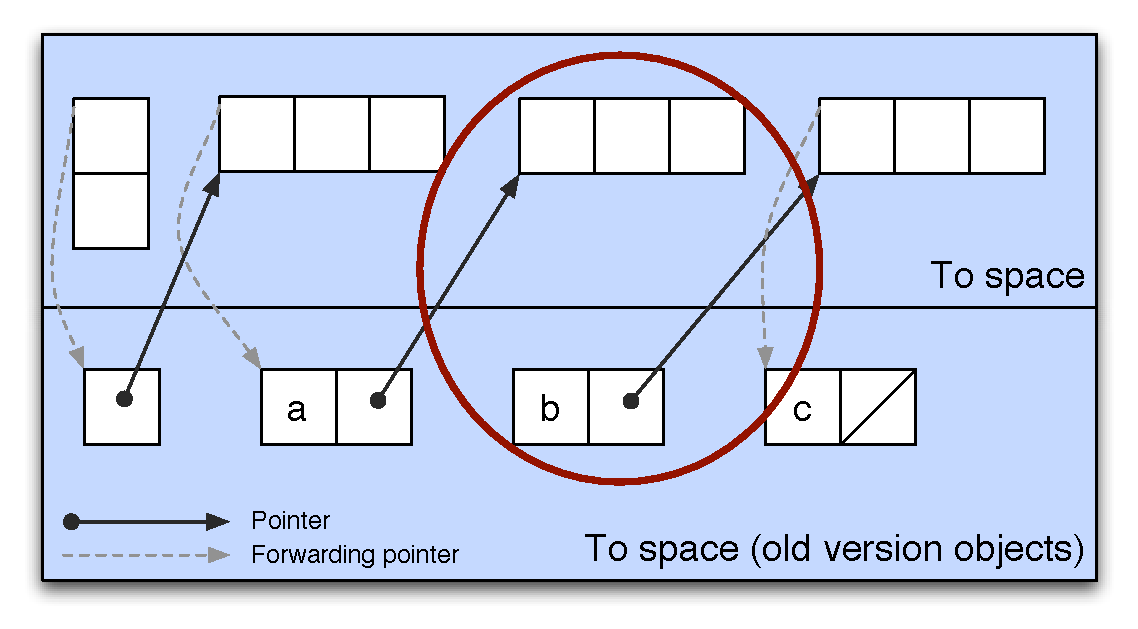
\includegraphics[scale=0.45]{images/singly-doubly/singly-doubly-transform-b-step-0}}%
% \only<5>{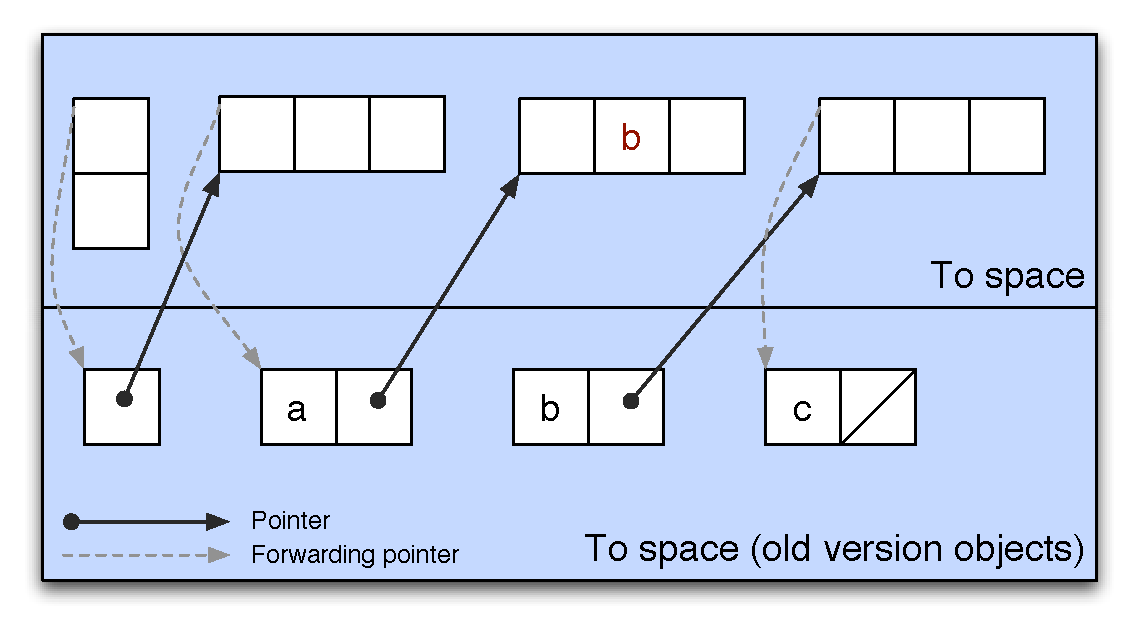
\includegraphics[scale=0.45]{images/singly-doubly/singly-doubly-transform-b-step-1}}%
% \only<6>{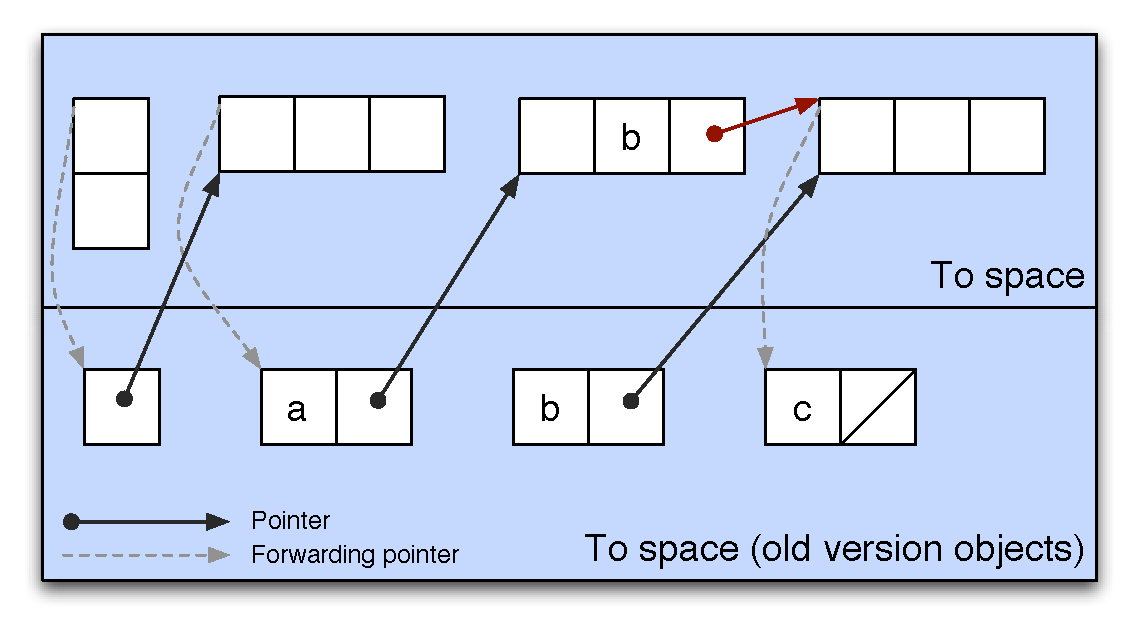
\includegraphics[scale=0.45]{images/singly-doubly/singly-doubly-transform-b-step-2}}%
% \only<7>{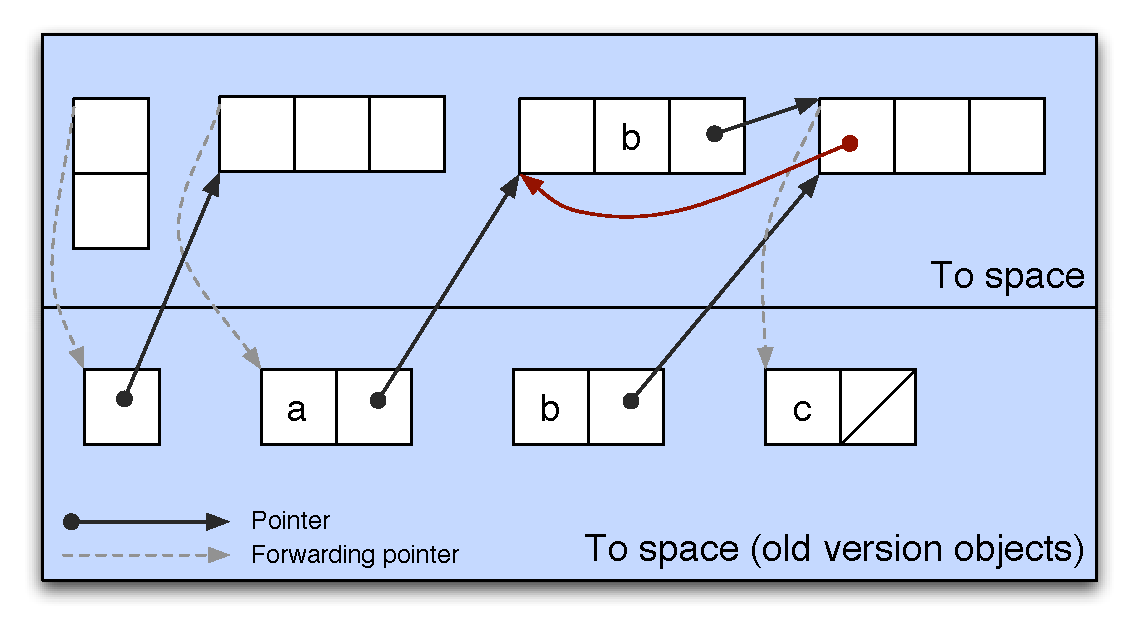
\includegraphics[scale=0.45]{images/singly-doubly/singly-doubly-transform-b-step-3}}%
% \only<8>{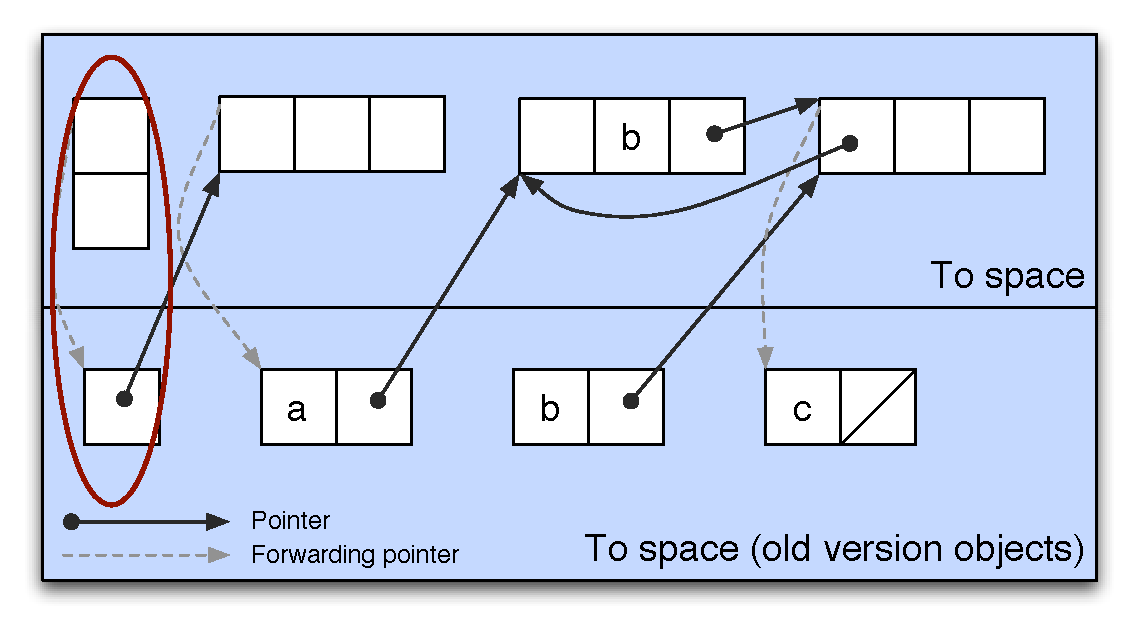
\includegraphics[scale=0.45]{images/singly-doubly/singly-doubly-transform-head-step-0}}%
% \only<9>{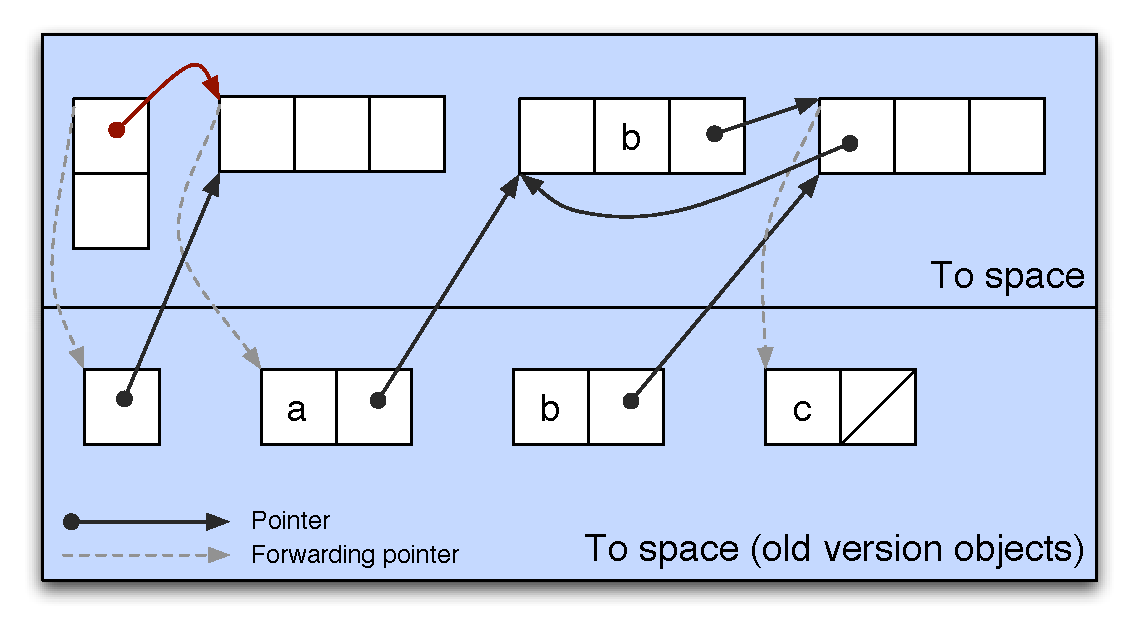
\includegraphics[scale=0.45]{images/singly-doubly/singly-doubly-transform-head-step-1}}%
% \only<10>{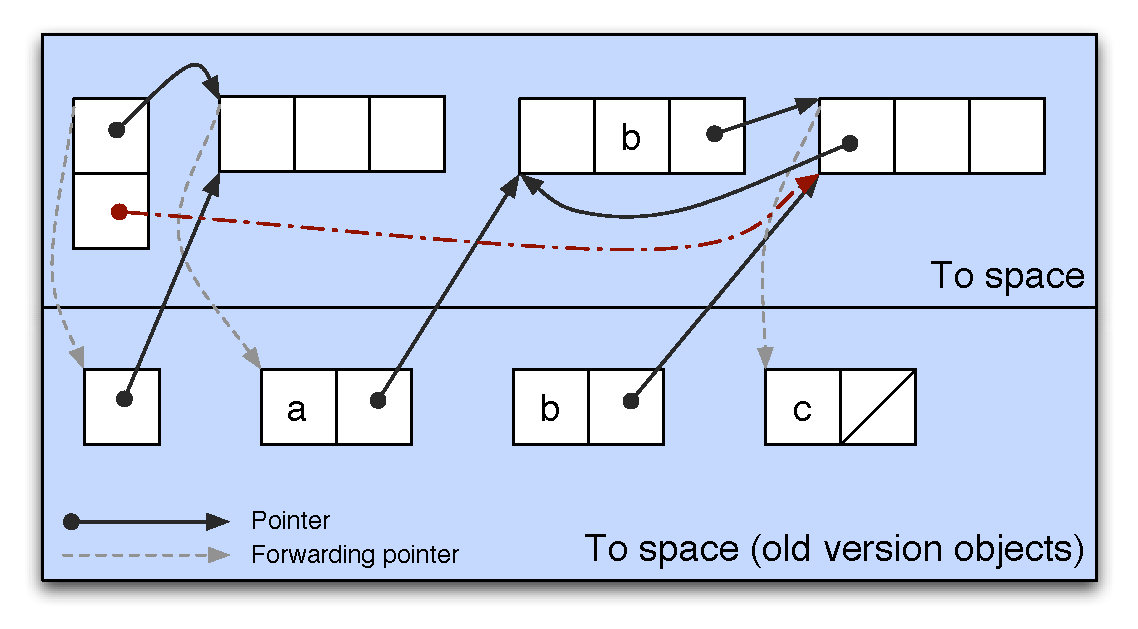
\includegraphics[scale=0.45]{images/singly-doubly/singly-doubly-transform-head-step-2}}%
% \only<11>{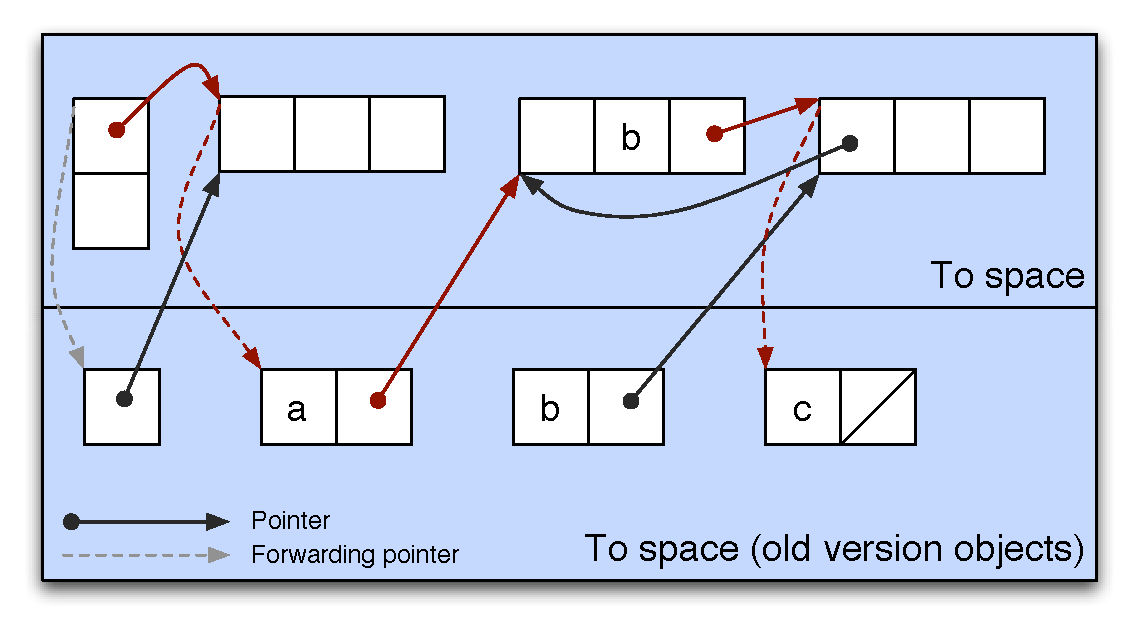
\includegraphics[scale=0.45]{images/singly-doubly/singly-doubly-transform-head-step-3-traverse-list}}%
% \only<12>{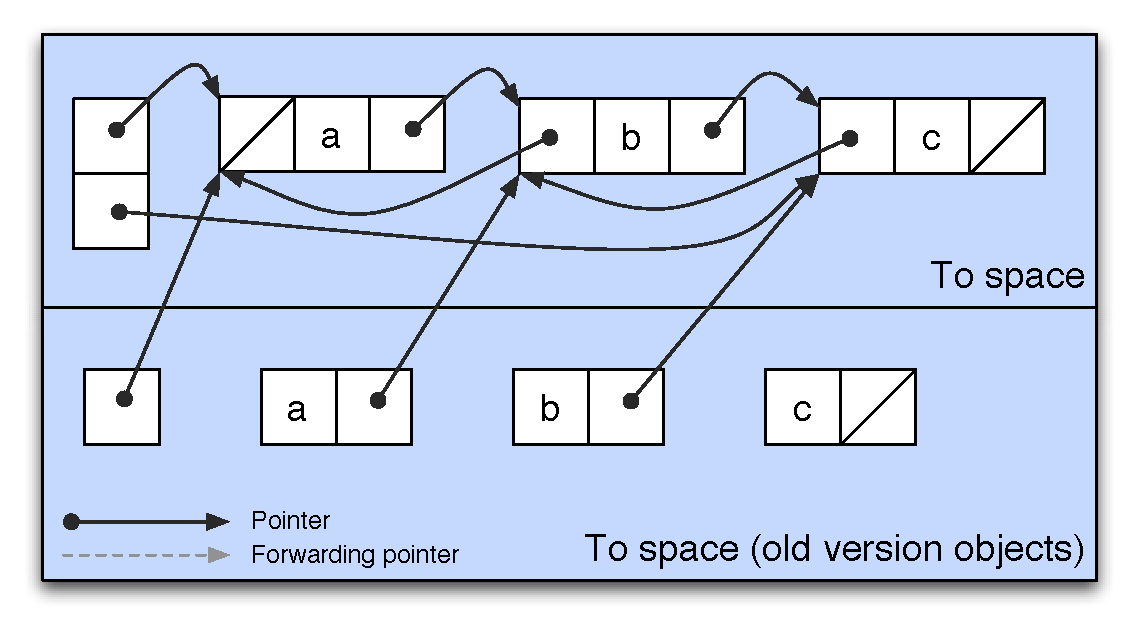
\includegraphics[scale=0.45]{images/singly-doubly/singly-doubly-transformed}}%
% \only<13>{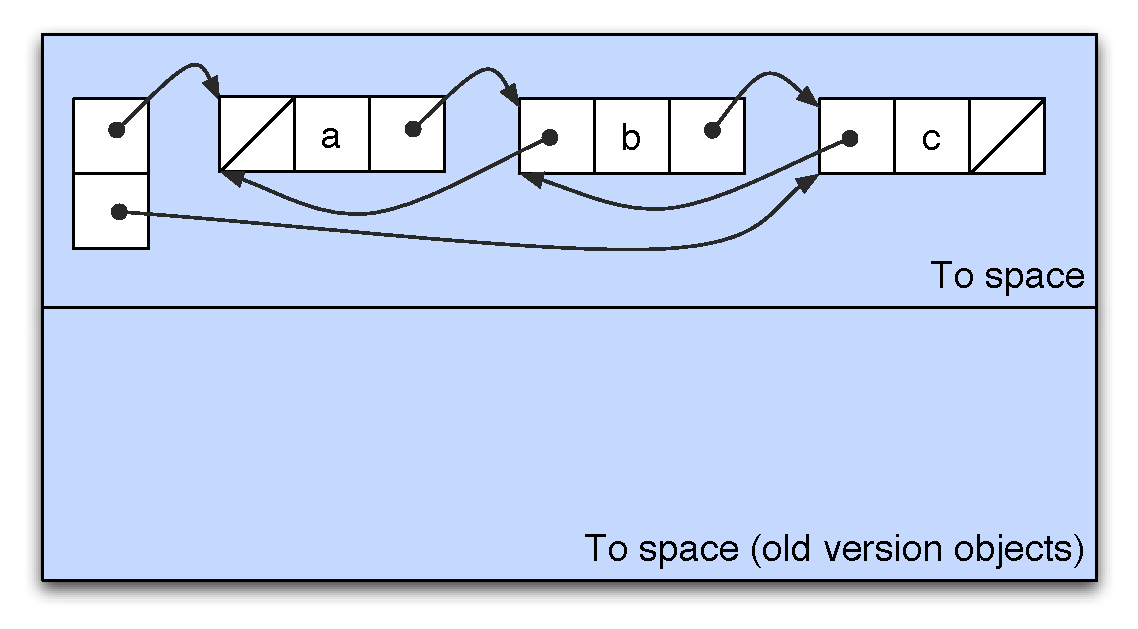
\includegraphics[scale=0.45]{images/singly-doubly/singly-doubly-transformed-final}}%
% \end{column}
% \begin{column}{0.37\paperwidth}%
% % Transform b, step 0
% \only<4>{%
% \begin{footnotesize}%
% \noindent {\tt jvolveObject(Node to,}\\
% {\tt\ \ \ \ old\_Node from) \{}\\
% {\tt\ \ to.data = from.data;}\\
% {\tt\ \ to.next = from.next;}\\
% {\tt\ \ if (to.next != null)}\\
% {\tt\ \ \ \ to.next.prev = to;}\\
% {\tt \}}
% \end{footnotesize}%
% }%
% % Transform b, step 1
% \only<5>{%
% \begin{footnotesize}%
% \noindent {\tt jvolveObject(Node to,}\\
% {\tt\ \ \ \ old\_Node from) \{}\\
% {\tt\ \ \colorbox{yellow}{to.data = from.data;}}\\
% {\tt\ \ to.next = from.next;}\\
% {\tt\ \ if (to.next != null)}\\
% {\tt\ \ \ \ to.next.prev = to;}\\
% {\tt \}}
% \end{footnotesize}%
% }%
% % Transform b, step 2
% \only<6>{%
% \begin{footnotesize}%
% \noindent {\tt jvolveObject(Node to,}\\
% {\tt\ \ \ \ old\_Node from) \{}\\
% {\tt\ \ to.data = from.data;}\\
% {\tt\ \ \colorbox{yellow}{to.next = from.next;}}\\
% {\tt\ \ if (to.next != null)}\\
% {\tt\ \ \ \ to.next.prev = to;}\\
% {\tt \}}
% \end{footnotesize}%
% }%
% % Transform b, step 3
% \only<7>{%
% \begin{footnotesize}%
% \noindent {\tt jvolveObject(Node to,}\\
% {\tt\ \ \ \ old\_Node from) \{}\\
% {\tt\ \ to.data = from.data;}\\
% {\tt\ \ to.next = from.next;}\\
% {\tt\ \ \colorbox{yellow}{if (to.next != null)}}\\
% {\tt\ \ \colorbox{yellow}{\ \ to.next.prev = to;}}\\
% {\tt \}}
% \end{footnotesize}%
% }%
% \end{column}
% \end{columns}
% \end{frame}

\begin{frame}[fragile]{Singly-linked to doubly-linked list}%{A Sub-title is optional}
\begin{columns}[c]
\begin{column}{0.67\paperwidth}
\only<1>{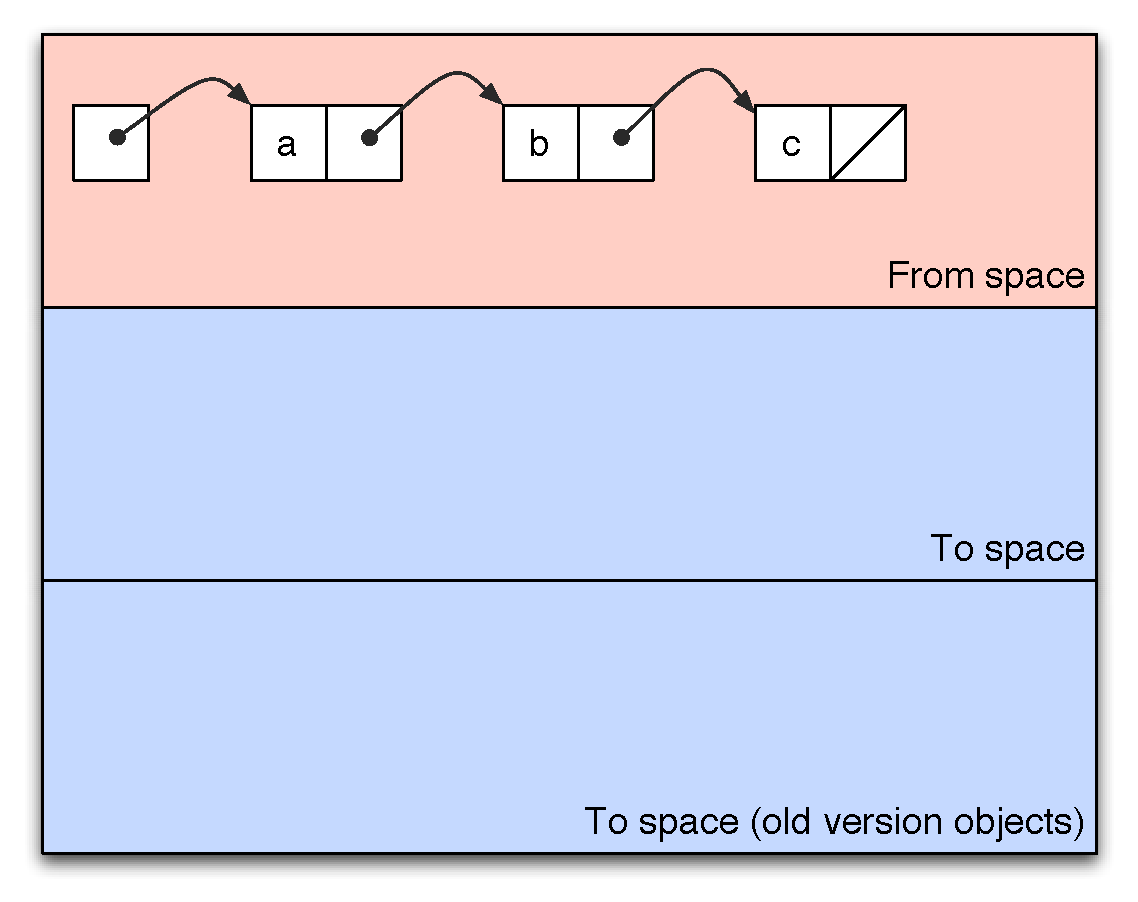
\includegraphics[scale=0.45]{images/singly-doubly/before-gc-copy}}%
\only<2>{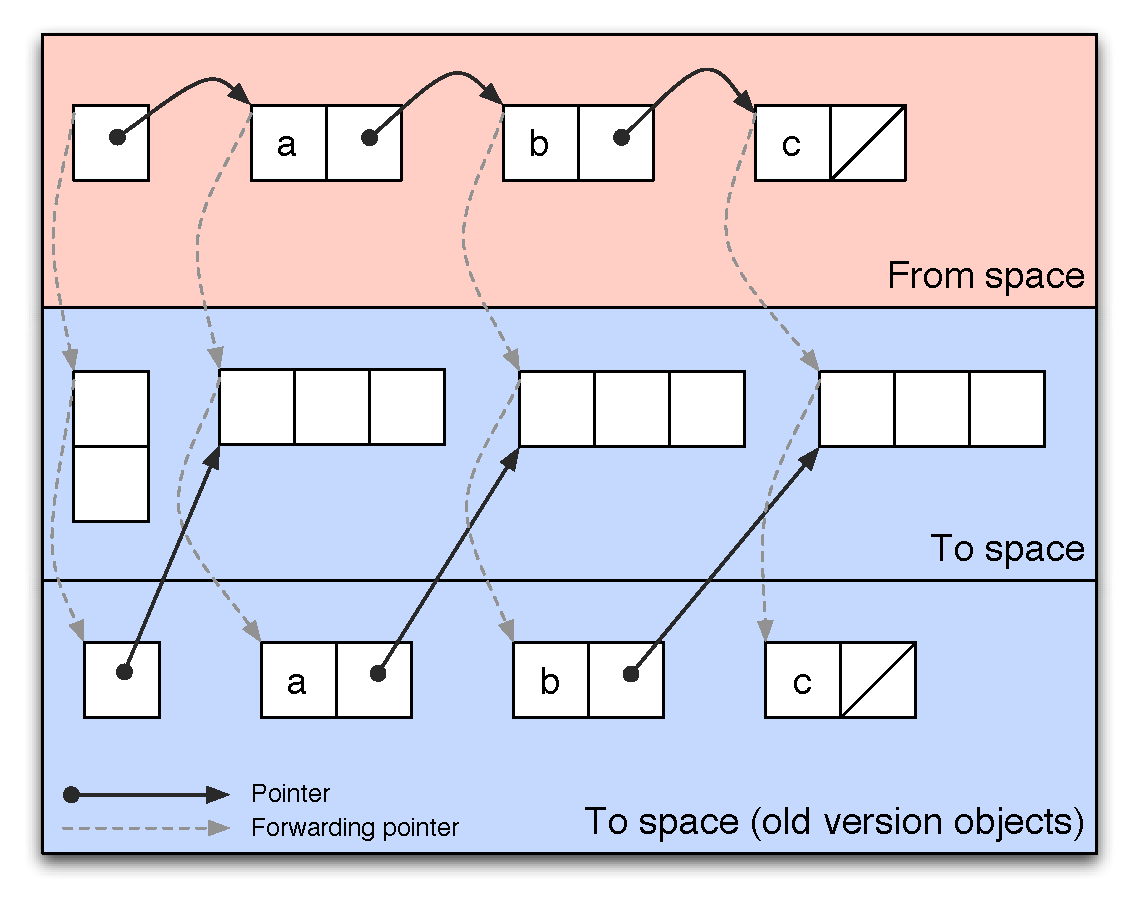
\includegraphics[scale=0.45]{images/singly-doubly/singly-doubly}}%
\only<3>{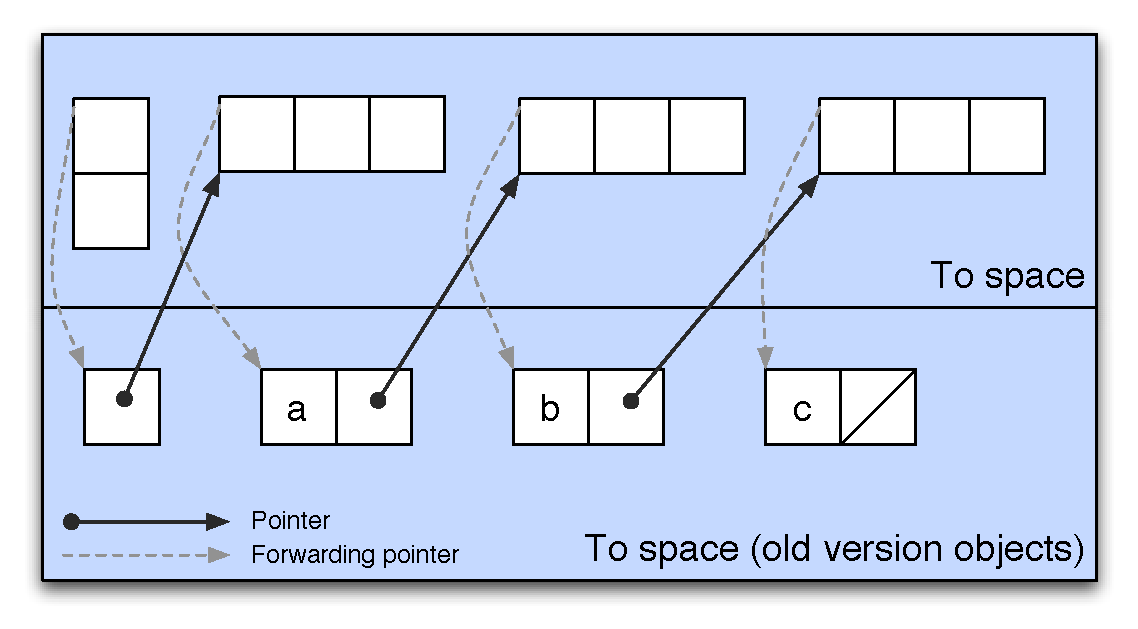
\includegraphics[scale=0.45]{images/singly-doubly/singly-doubly-before-transform}}%
\only<4>{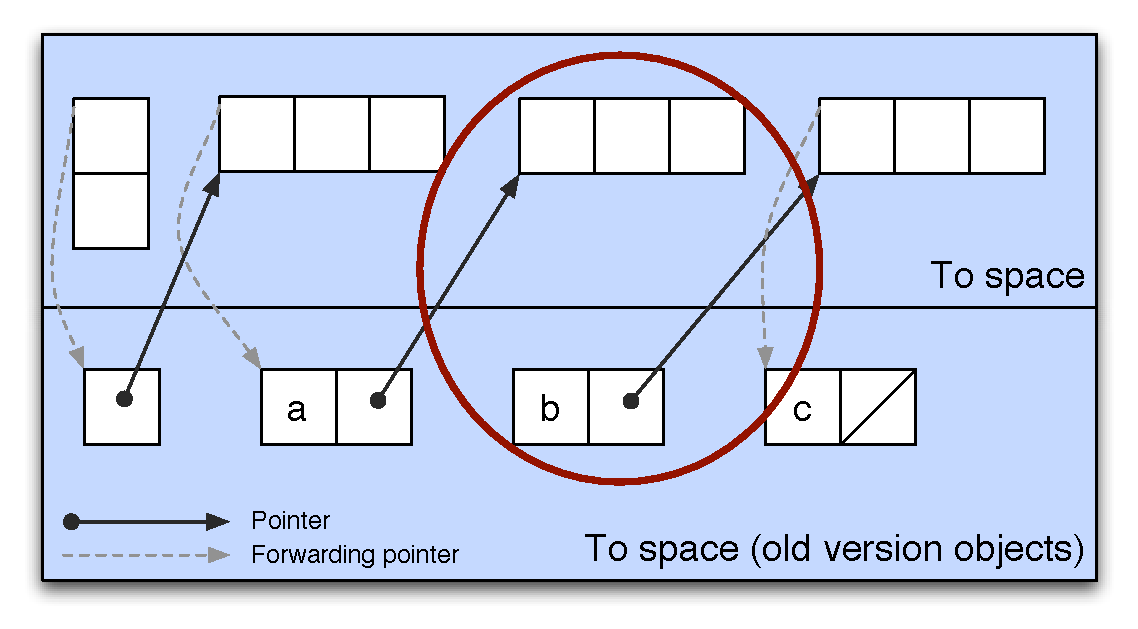
\includegraphics[scale=0.45]{images/singly-doubly/singly-doubly-transform-b-step-0}}%
\only<5>{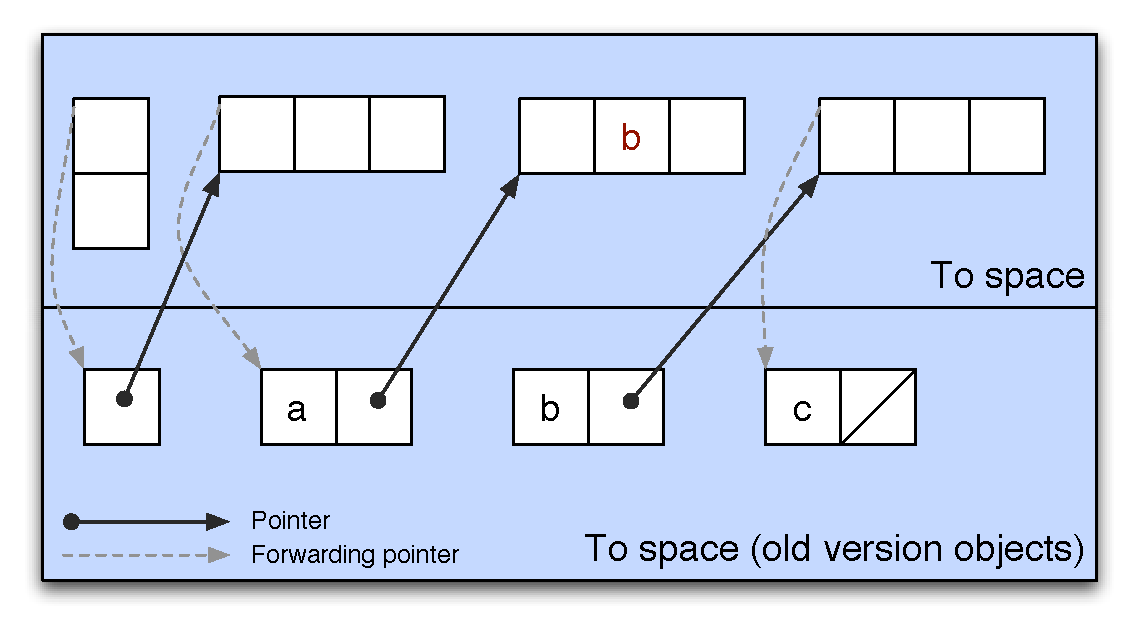
\includegraphics[scale=0.45]{images/singly-doubly/singly-doubly-transform-b-step-1}}%
\only<6>{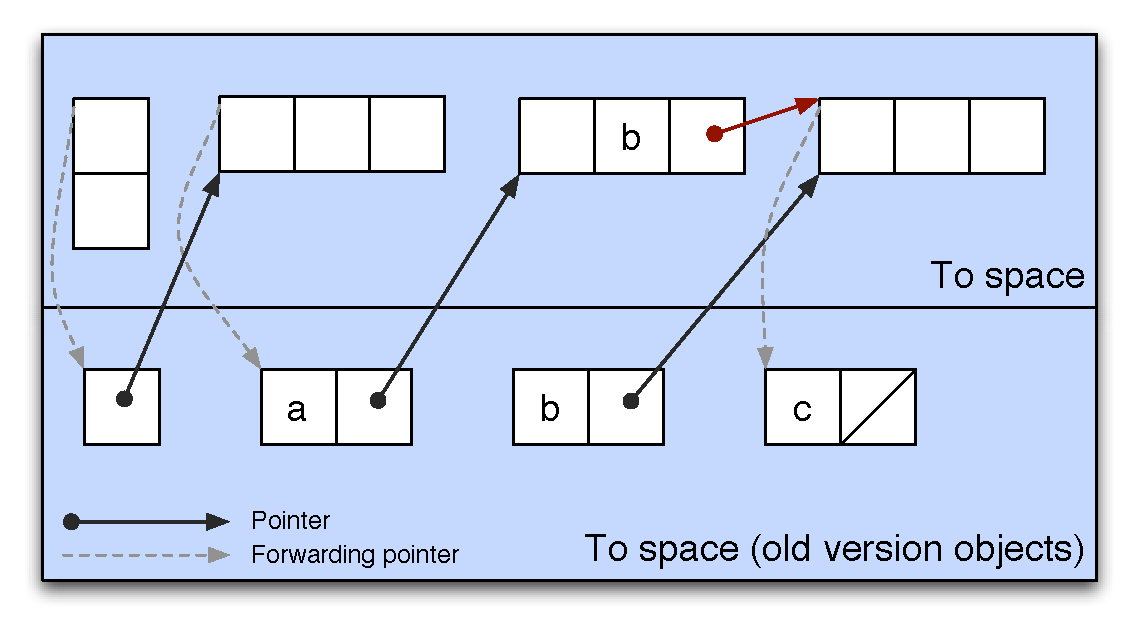
\includegraphics[scale=0.45]{images/singly-doubly/singly-doubly-transform-b-step-2}}%
\only<7>{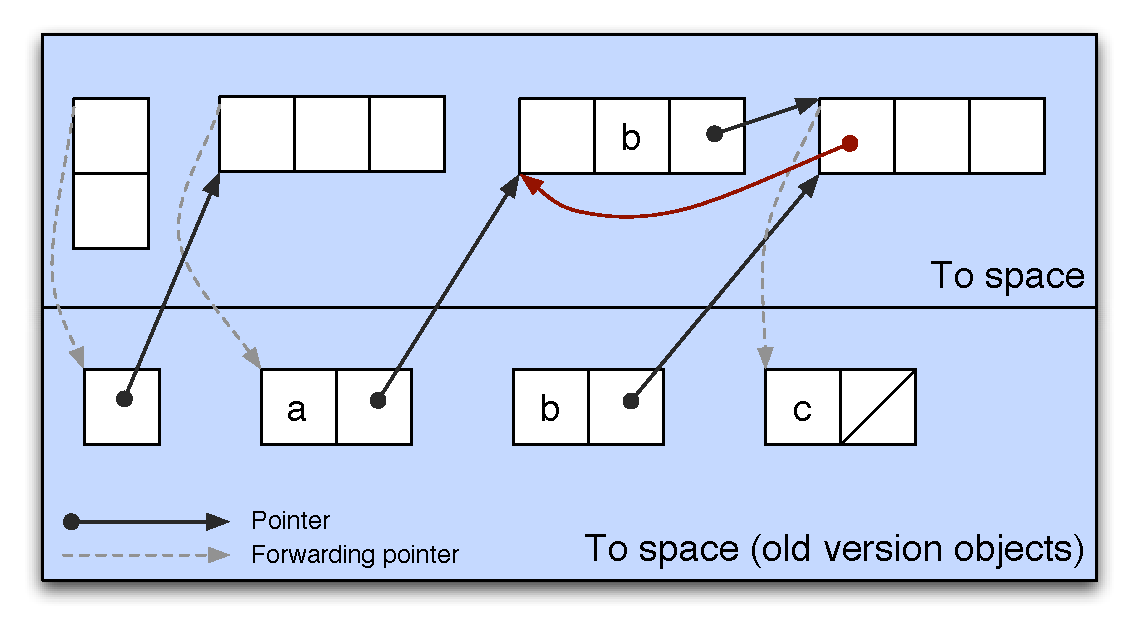
\includegraphics[scale=0.45]{images/singly-doubly/singly-doubly-transform-b-step-3}}%
\only<8>{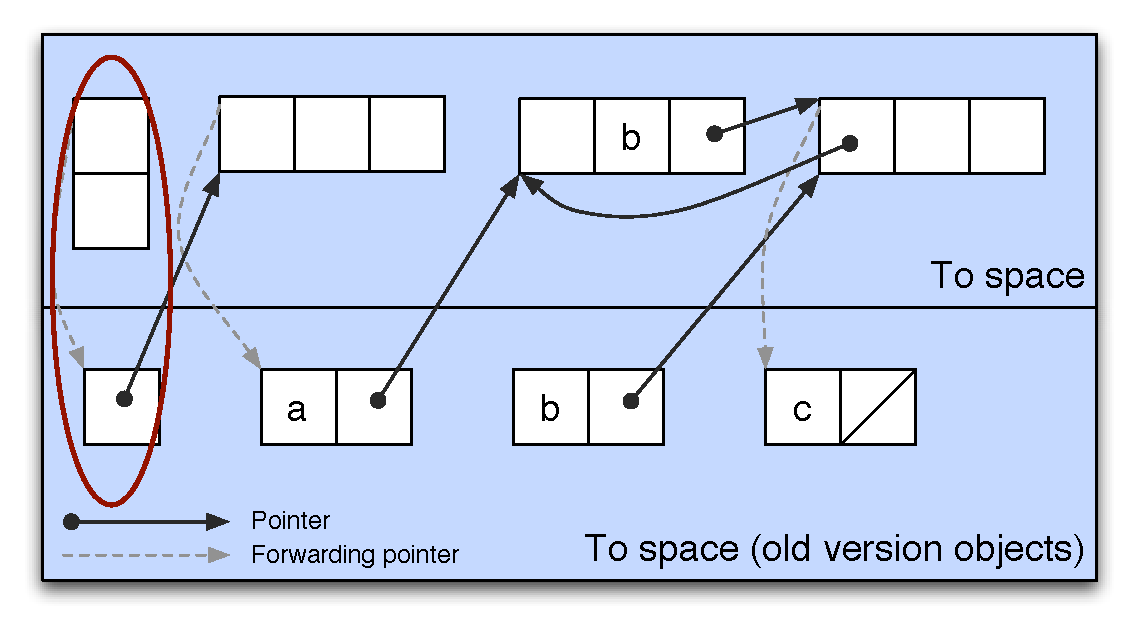
\includegraphics[scale=0.45]{images/singly-doubly/singly-doubly-transform-head-step-0}}%
\only<9>{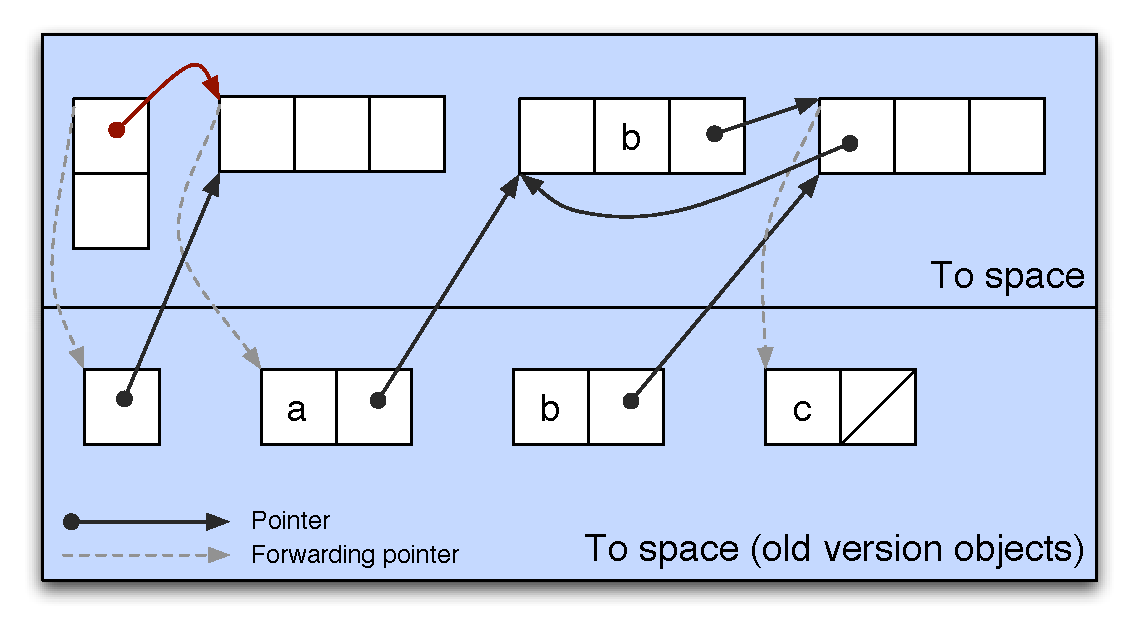
\includegraphics[scale=0.45]{images/singly-doubly/singly-doubly-transform-head-step-1}}%
\only<10>{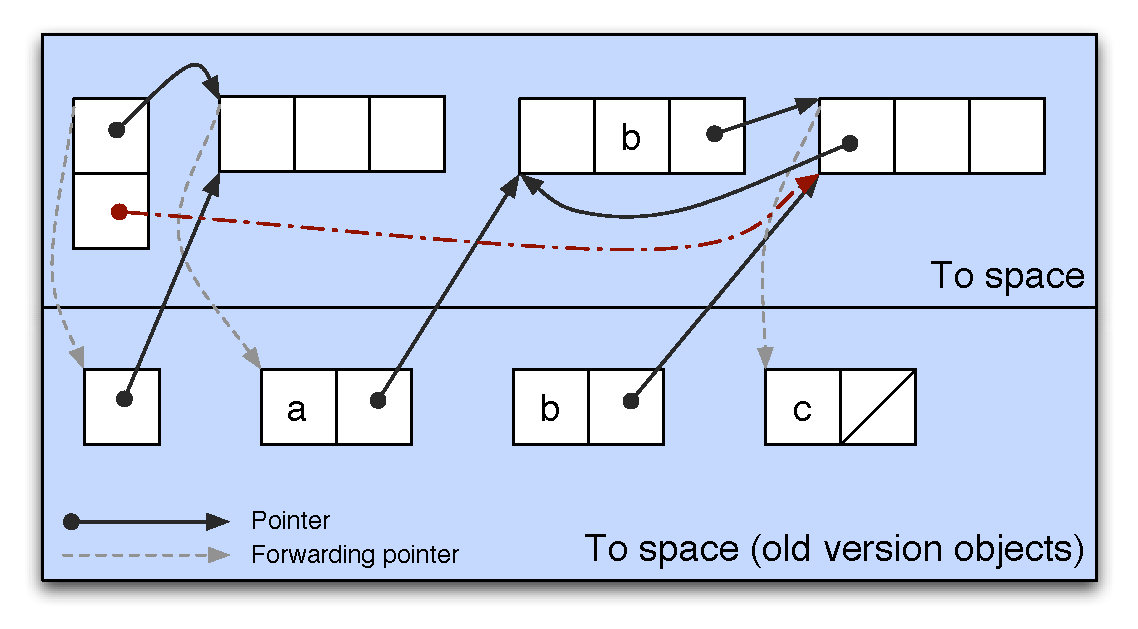
\includegraphics[scale=0.45]{images/singly-doubly/singly-doubly-transform-head-step-2}}%
\end{column}
\begin{column}{0.37\paperwidth}%
% Transform b, step 0
\only<4>{%
\begin{footnotesize}%
\noindent {\tt jvolveObject(Node to,}\\
{\tt\ \ \ \ old\_Node from) \{}\\
{\tt\ \ to.data = from.data;}\\
{\tt\ \ to.next = from.next;}\\
{\tt\ \ if (to.next != null)}\\
{\tt\ \ \ \ to.next.prev = to;}\\
{\tt \}}
\end{footnotesize}%
}%
% Transform b, step 1
\only<5>{%
\begin{footnotesize}%
\noindent {\tt jvolveObject(Node to,}\\
{\tt\ \ \ \ old\_Node from) \{}\\
{\tt\ \ \colorbox{yellow}{to.data = from.data;}}\\
{\tt\ \ to.next = from.next;}\\
{\tt\ \ if (to.next != null)}\\
{\tt\ \ \ \ to.next.prev = to;}\\
{\tt \}}
\end{footnotesize}%
}%
% Transform b, step 2
\only<6>{%
\begin{footnotesize}%
\noindent {\tt jvolveObject(Node to,}\\
{\tt\ \ \ \ old\_Node from) \{}\\
{\tt\ \ to.data = from.data;}\\
{\tt\ \ \colorbox{yellow}{to.next = from.next;}}\\
{\tt\ \ if (to.next != null)}\\
{\tt\ \ \ \ to.next.prev = to;}\\
{\tt \}}
\end{footnotesize}%
}%
% Transform b, step 3
\only<7>{%
\begin{footnotesize}%
\noindent {\tt jvolveObject(Node to,}\\
{\tt\ \ \ \ old\_Node from) \{}\\
{\tt\ \ to.data = from.data;}\\
{\tt\ \ to.next = from.next;}\\
{\tt\ \ \colorbox{yellow}{if (to.next != null)}}\\
{\tt\ \ \colorbox{yellow}{\ \ to.next.prev = to;}}\\
{\tt \}}
\end{footnotesize}%
}%
\end{column}
\end{columns}
\end{frame}

\begin{frame}[fragile]{Finding the list's tail}%{A Sub-title is optional}
\begin{minipage}{0.95\textwidth}
% \lstset{moredelim=[is][\color{structure.fg!75!black}]{>}{<}}
\begin{lstlisting}[numbers=none,basicstyle=\footnotesize\ttfamily]
Node prev = null;
Node current = from.head;
while (current != null) {
  prev = current;
\end{lstlisting}\vspace{-2ex}
\begin{lstlisting}[numbers=none,basicstyle=\footnotesize\ttfamily,backgroundcolor=\color{yellow}]
  if (! VM.is_transformed(current)) {
    r0_Node current_old = VM.old_version_object(current);
    current = current_old.next;
\end{lstlisting}\vspace{-2ex}
\begin{lstlisting}[numbers=none,basicstyle=\footnotesize\ttfamily]
  } else {
    current = current.next;
  }
}
to.tail = prev;
\end{lstlisting}
\end{minipage}
\end{frame}

\begin{frame}[fragile]{Singly-linked to doubly-linked list}%{A Sub-title is optional}
\begin{columns}[c]
\begin{column}{0.67\paperwidth}
\only<1>{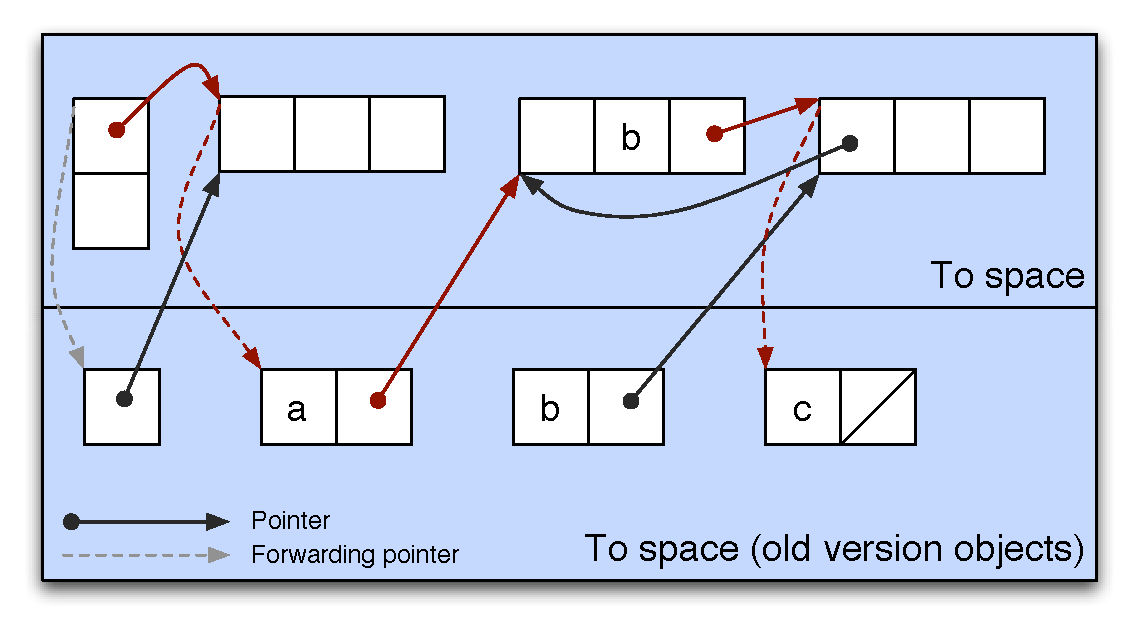
\includegraphics[scale=0.45]{images/singly-doubly/singly-doubly-transform-head-step-3-traverse-list}}%
\only<2>{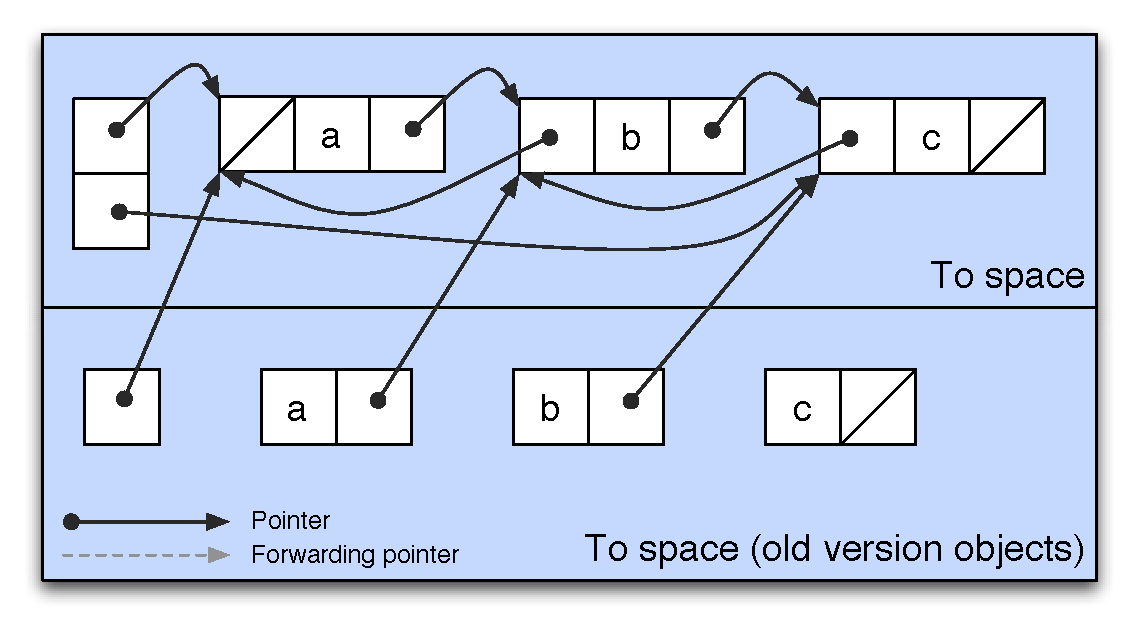
\includegraphics[scale=0.45]{images/singly-doubly/singly-doubly-transformed}}%
\only<3>{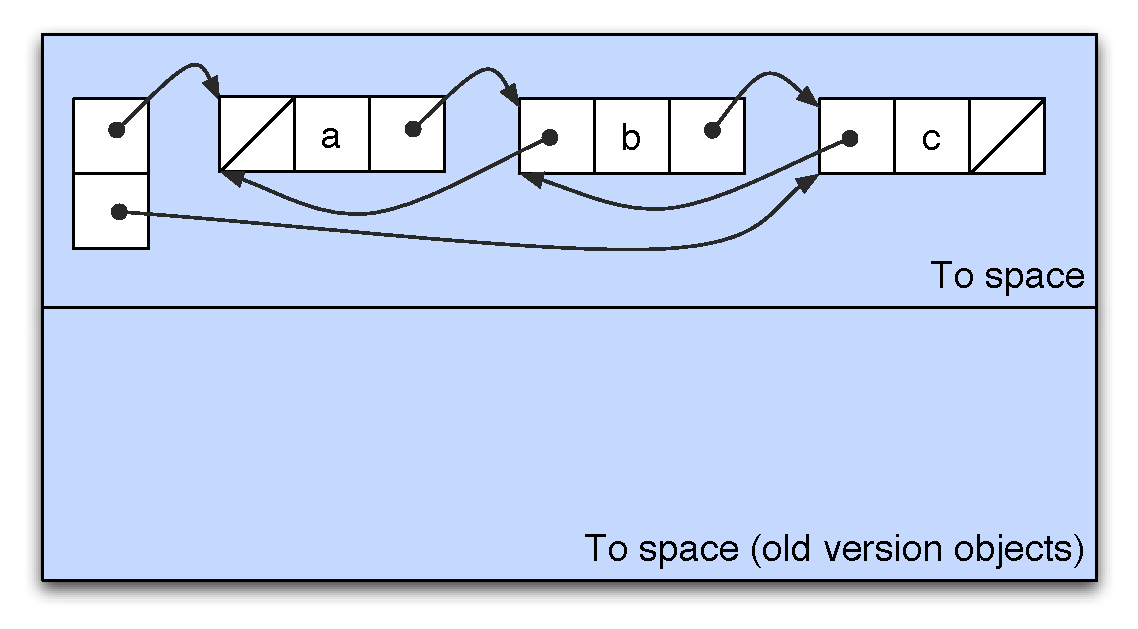
\includegraphics[scale=0.45]{images/singly-doubly/singly-doubly-transformed-final}}%
\end{column}
\begin{column}{0.37\paperwidth}%
\end{column}
\end{columns}
\end{frame}
